\subsection{Алгоритм Беллмана-Форда}
\label{subsec:bellman-ford-subsection}

Алгоритм Беллмана-Форда --- це алгоритм найкоротшого шляху з одним джерелом, що означає, що він знаходить найкоротший шлях від однієї вихідної вершини до всіх інших вершин зваженого графа. Він був розроблений Річардом Беллманом і Лестером Фордом у 1950-х роках.

Алгоритм працює, підтримуючи список найкоротших відстаней від вихідної вершини до кожної вершини графа. Спочатку найкоротша відстань до самої вихідної вершини дорівнює 0, а відстань до всіх інших вершин дорівнює нескінченності.

Потім алгоритм ітерує всі ребра графа, послаблюючи їх по черзі. Послаблення ребра означає оновлення найкоротшої відстані до вершини на іншому кінці ребра, якщо знайдено коротший шлях до цієї вершини. Цей процес повторюється V-1 раз, де V - кількість вершин у графі, щоб переконатися, що всі можливі шляхи були досліджені.

Якщо після V-1 ітерацій залишаються ребра, які можна послабити, це означає, що граф містить цикл з від'ємною вагою. Цикл з від'ємною вагою - це цикл ребер у графі, сумарна вага яких від'ємна, і такий цикл може призвести до неправильних результатів роботи алгоритму, оскільки він може призвести до нескінченного циклу зменшення відстаней. Якщо виявлено цикл з від'ємною вагою, алгоритм повідомляє, що граф не містить найкоротших шляхів.

Часова складність алгоритму Беллмана-Форда становить O(V * E), де V - кількість вершин, а E - кількість ребер у графі. Це робить його повільнішим за алгоритм Дейкстри, але він здатен обробляти графи з ребрами з від'ємною вагою, чого не може алгоритм Дейкстри.\\

\begin{figure}[!htp]
    \centering
    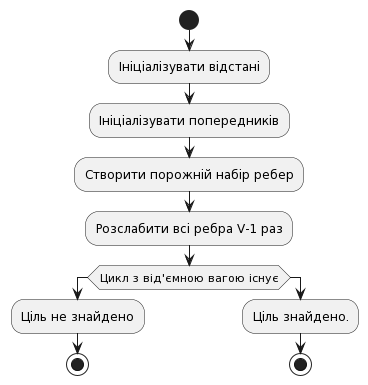
\includegraphics[scale=0.7]{content/chapters/2-implementation-methods/assets/img/bellman-ford_algorithm.png}
    \caption{Блок-схема алгоритму Беллмана-Форда}
    \label{fig:bellman-ford}
\end{figure}

Переваги:
\begin{itemize}
    \item Він може обробляти графи з ребрами з від'ємною вагою, на відміну від алгоритму Дейкстри.
    \item Може виявляти цикли з від'ємною вагою у графі.
    \item Простий у реалізації.
\end{itemize}

Недоліки:
\begin{itemize}
    \item Його часова складність становить O(V * E), що може зробити його повільним для великих графів.
    \item Він не може працювати з графами з циклами від'ємної ваги, оскільки застрягне у нескінченному циклі зменшення відстаней.
\end{itemize}
